% Options for packages loaded elsewhere
\PassOptionsToPackage{unicode}{hyperref}
\PassOptionsToPackage{hyphens}{url}
\PassOptionsToPackage{dvipsnames,svgnames*,x11names*}{xcolor}
%
\documentclass[
  10pt,
  ignorenonframetext,
  aspectratio=43,
]{beamer}
\usepackage{pgfpages}
\setbeamertemplate{caption}[numbered]
\setbeamertemplate{caption label separator}{: }
\setbeamercolor{caption name}{fg=normal text.fg}
\beamertemplatenavigationsymbolsempty

%%
%%% Definition of colors
%%% Source: https://latexcolor.com/
\definecolor{blanchedalmond}{rgb}{1.0, 0.92, 0.8}
\definecolor{blond}{rgb}{0.98, 0.94, 0.75}
%%% End of definition of colors
%%

% Prevent slide breaks in the middle of a paragraph
\widowpenalties 1 10000
\raggedbottom
\usepackage{lmodern}
\usepackage{amssymb,amsmath}
\usepackage{ifxetex,ifluatex}
\ifnum 0\ifxetex 1\fi\ifluatex 1\fi=0 % if pdftex
  \usepackage[T1]{fontenc}
  \usepackage[utf8]{inputenc}
  \usepackage{textcomp} % provide euro and other symbols
\else % if luatex or xetex
  \usepackage{unicode-math}
  \defaultfontfeatures{Scale=MatchLowercase}
  \defaultfontfeatures[\rmfamily]{Ligatures=TeX,Scale=1}
  \setmainfont[]{Myriad Pro}
  \ifxetex
    \usepackage{xeCJK}
    \setCJKmainfont[ItalicFont=AR PL UKai TW]{AR UDJingXiHeiPU30}
  \fi
  \ifluatex
    \usepackage[]{luatexja-fontspec}
    \setmainjfont[ItalicFont=AR PL UKai TW]{AR UDJingXiHeiPU30}
  \fi
\fi
\usetheme[]{metropolis}
\usecolortheme{default}
\usefonttheme{serif} % use mainfont rather than sansfont for slide text
% Use upquote if available, for straight quotes in verbatim environments
\IfFileExists{upquote.sty}{\usepackage{upquote}}{}
\IfFileExists{microtype.sty}{% use microtype if available
  \usepackage[]{microtype}
  \UseMicrotypeSet[protrusion]{basicmath} % disable protrusion for tt fonts
}{}
\makeatletter
\@ifundefined{KOMAClassName}{% if non-KOMA class
  \IfFileExists{parskip.sty}{%
    \usepackage{parskip}
  }{% else
    \setlength{\parindent}{0pt}
    \setlength{\parskip}{6pt plus 2pt minus 1pt}}
}{% if KOMA class
  \KOMAoptions{parskip=half}}
\makeatother
\usepackage{xcolor}
\IfFileExists{xurl.sty}{\usepackage{xurl}}{} % add URL line breaks if available
\IfFileExists{bookmark.sty}{\usepackage{bookmark}}{\usepackage{hyperref}}
\hypersetup{
  pdftitle={The Fall of the Labor Share and the Rise of Superstar Firms},
  pdfauthor={Yu-Hsin Ho},
  colorlinks=true,
  linkcolor=Maroon,
  filecolor=Maroon,
  citecolor=Blue,
  urlcolor=red,
  pdfcreator={LaTeX via pandoc}}
\urlstyle{same} % disable monospaced font for URLs
\newif\ifbibliography
\usepackage{listings}
\newcommand{\passthrough}[1]{#1}
\lstset{defaultdialect=sh}
\lstset{framexleftmargin=0mm, frame=trBL,backgroundcolor=\color{blanchedalmond!5},numbers=left,numberstyle=\scriptsize,basicstyle=\small}
\lstset{aboveskip=5mm,belowskip=5mm,xleftmargin=20pt,xrightmargin=5pt}
% \lstset{prebreak={\raisebox{0ex}[0ex][0ex]}}
% \lstset{postbreak={\raisebox{0ex}[0ex][0ex]\space}}
\lstset{breaklines=true,breakatwhitespace=true}
\usepackage{longtable,booktabs}
\usepackage{graphicx,grffile}
\makeatletter
\def\maxwidth{\ifdim\Gin@nat@width>\linewidth\linewidth\else\Gin@nat@width\fi}
\def\maxheight{\ifdim\Gin@nat@height>\textheight\textheight\else\Gin@nat@height\fi}
\makeatother
% Scale images if necessary, so that they will not overflow the page
% margins by default, and it is still possible to overwrite the defaults
% using explicit options in \includegraphics[width, height, ...]{}
\setkeys{Gin}{width=\maxwidth,height=\maxheight,keepaspectratio}
% Set default figure placement to htbp
\makeatletter
\def\fps@figure{htbp}
\makeatother
\setlength{\emergencystretch}{3em} % prevent overfull lines
\providecommand{\tightlist}{%
  \setlength{\itemsep}{0pt}\setlength{\parskip}{0pt}}
\setcounter{secnumdepth}{-\maxdimen} % remove section numbering

%
% When using babel or polyglossia with biblatex, loading csquotes is recommended 
% to ensure that quoted texts are typeset according to the rules of your main language.
%
\usepackage{csquotes}

%
% blockquote
%
\definecolor{blockquote-border}{RGB}{221,221,221}
\definecolor{blockquote-text}{RGB}{89,89,89}
\usepackage{mdframed}
\newmdenv[rightline=false,bottomline=false,topline=false,linewidth=3pt,linecolor=blockquote-border,skipabove=\parskip]{customblockquote}
\renewenvironment{quote}{\begin{customblockquote}\list{}{\rightmargin=0em\leftmargin=0em}%
\item\relax\color{blockquote-text}\ignorespaces}{\unskip\unskip\endlist\end{customblockquote}}

%
% Source Sans Pro as the de­fault font fam­ily
% Source Code Pro for monospace text
%
% 'default' option sets the default 
% font family to Source Sans Pro, not \sfdefault.
%

\usepackage{adjustbox}
\usepackage{booktabs}
\linespread{1.2}
\usepackage[font={footnotesize}]{caption}

\title{The Fall of the Labor Share and the Rise of Superstar Firms}
\subtitle{Autor, David, Dorn, David, Katz, Lawrence F, Patterson,
Christina, and Van Reenen, John, The Quarterly Journal of Economics, 135
(2020), 645--709.}
\author{Yu-Hsin Ho}
\date{May 16, 2022}
\institute{Department of Economics, National Taiwan University}

\begin{document}
\frame{\titlepage}

\hypertarget{introduction}{%
\section{Introduction}\label{introduction}}

\begin{frame}{Introduction}
\begin{figure}
\centering
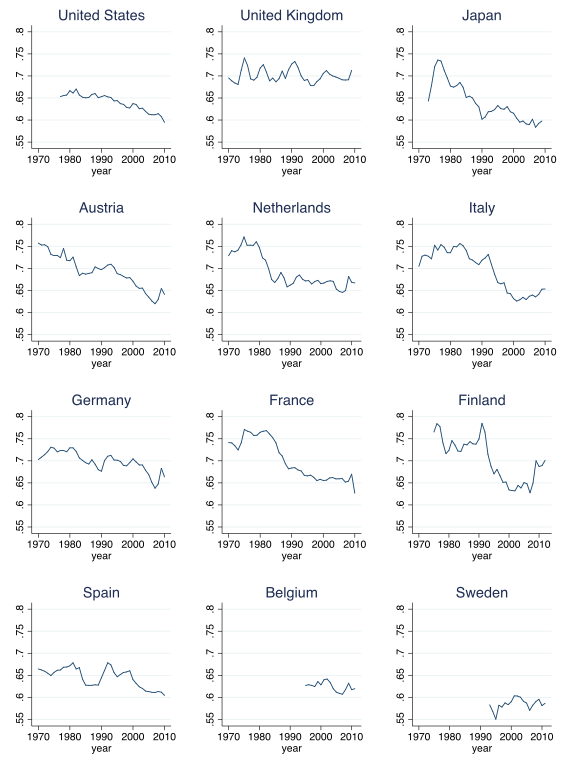
\includegraphics[width=0.5\textwidth,height=\textheight]{./images/Pasted image 20220516142524.png}
\caption{International Comparison: Labor Share by Country}
\end{figure}
\end{frame}

\begin{frame}
Decline of labor share is a global phenomenon, why?

\begin{itemize}
\tightlist
\item
  Relative low price of capital
\item
  International trade
\item
  \textbf{Rise of superstar firms}

  \begin{itemize}
  \tightlist
  \item
    High monopoly profit (markup)
  \item
    Winner takes most / Network effects
  \item
    High initial investment (sunk cost)
  \end{itemize}
\end{itemize}
\end{frame}

\begin{frame}{7 Empirical Facts}
\protect\hypertarget{empirical-facts}{}
\begin{enumerate}
\item
  Sales concentration
\item
  More concentration, larger decline in labor share.
\item
  Main force: Reallocation of sales between firms
\item
  More concentration, higher reallocation effect
\item
  Growth of productivity and innovation leads to concentration
\item
  Larger firms, higher markup
\item
  Decline in labor share is an international phenomenon
\end{enumerate}
\end{frame}

\hypertarget{conceptual-model}{%
\section{Conceptual Model}\label{conceptual-model}}

\begin{frame}{Conceptual Model}
Consider a Cobb-Douglas Production Function: \[
Y_i = z_i L_i^{\alpha^L} K_i^{1 - \alpha^L}
\]

And define labor share for each industry \(i\): \[
S_i \equiv \frac{w L_i}{P_i Y_i} = \frac{\alpha^L}{m_i}
\]

where markup \(m_i = \frac{P_i}{c_i}\), and economy-wide parameters
\(\{\alpha^L, w\}\)

Empirically, we look at payroll over total sales.
\end{frame}

\begin{frame}{Toughness in the market competition}
\protect\hypertarget{toughness-in-the-market-competition}{}
Tough competition leads to\ldots{}

\begin{enumerate}
\item
  Overall reduction in markup: With-in firm effect
\item
  Reallocation of market share to large firms: Between-firm effect

  With increased weight for firms with lower labor share, weighted
  average labor share will decline.
\end{enumerate}

For observed declining labor share, (2) must dominate (1).
\end{frame}

\hypertarget{data}{%
\section{Data}\label{data}}

\begin{frame}{Data}
\begin{enumerate}
\tightlist
\item
  U.S. Economic Census: 1982-2012

  \begin{enumerate}
  \tightlist
  \item
    annual payroll; output (sales); employment;
  \item
    per-establishment micro data
  \end{enumerate}
\item
  EU KLEMS: industry-level OECD data set, 1980\textasciitilde{}
\item
  UN Comtrade Database: 1992-2012

  \begin{enumerate}
  \tightlist
  \item
    Import time series from six country groups for each industry.
  \end{enumerate}
\item
  CompNet: Industry-level data from 14 EU countries, 2000-2012
\item
  BVD Orbis: Firm-level panel data from 6 EU countries.
\end{enumerate}
\end{frame}

\begin{frame}{Index Definitions}
\protect\hypertarget{index-definitions}{}
\begin{block}{Labor Share}
\protect\hypertarget{labor-share}{}
\[
S = \frac{\text{Payroll}}{\text{Total Sales or Value Added}}
\]
\end{block}

\begin{block}{Concentration (Industry-level)}
\protect\hypertarget{concentration-industry-level}{}
\begin{enumerate}
\tightlist
\item
  CR4: \(\frac{\text{top 4 firms total sale}}{\text{total sales}}\)
\item
  CR20: \(\frac{\text{top 20 firms total sale}}{\text{total sales}}\)
\item
  Herfindahl-Hirschman Index (HHI): Sum of square of top-50 market share
\end{enumerate}
\end{block}
\end{frame}

\hypertarget{empirical-findings}{%
\section{Empirical Findings}\label{empirical-findings}}

\begin{frame}{Empirical Findings}
\begin{figure}
\centering
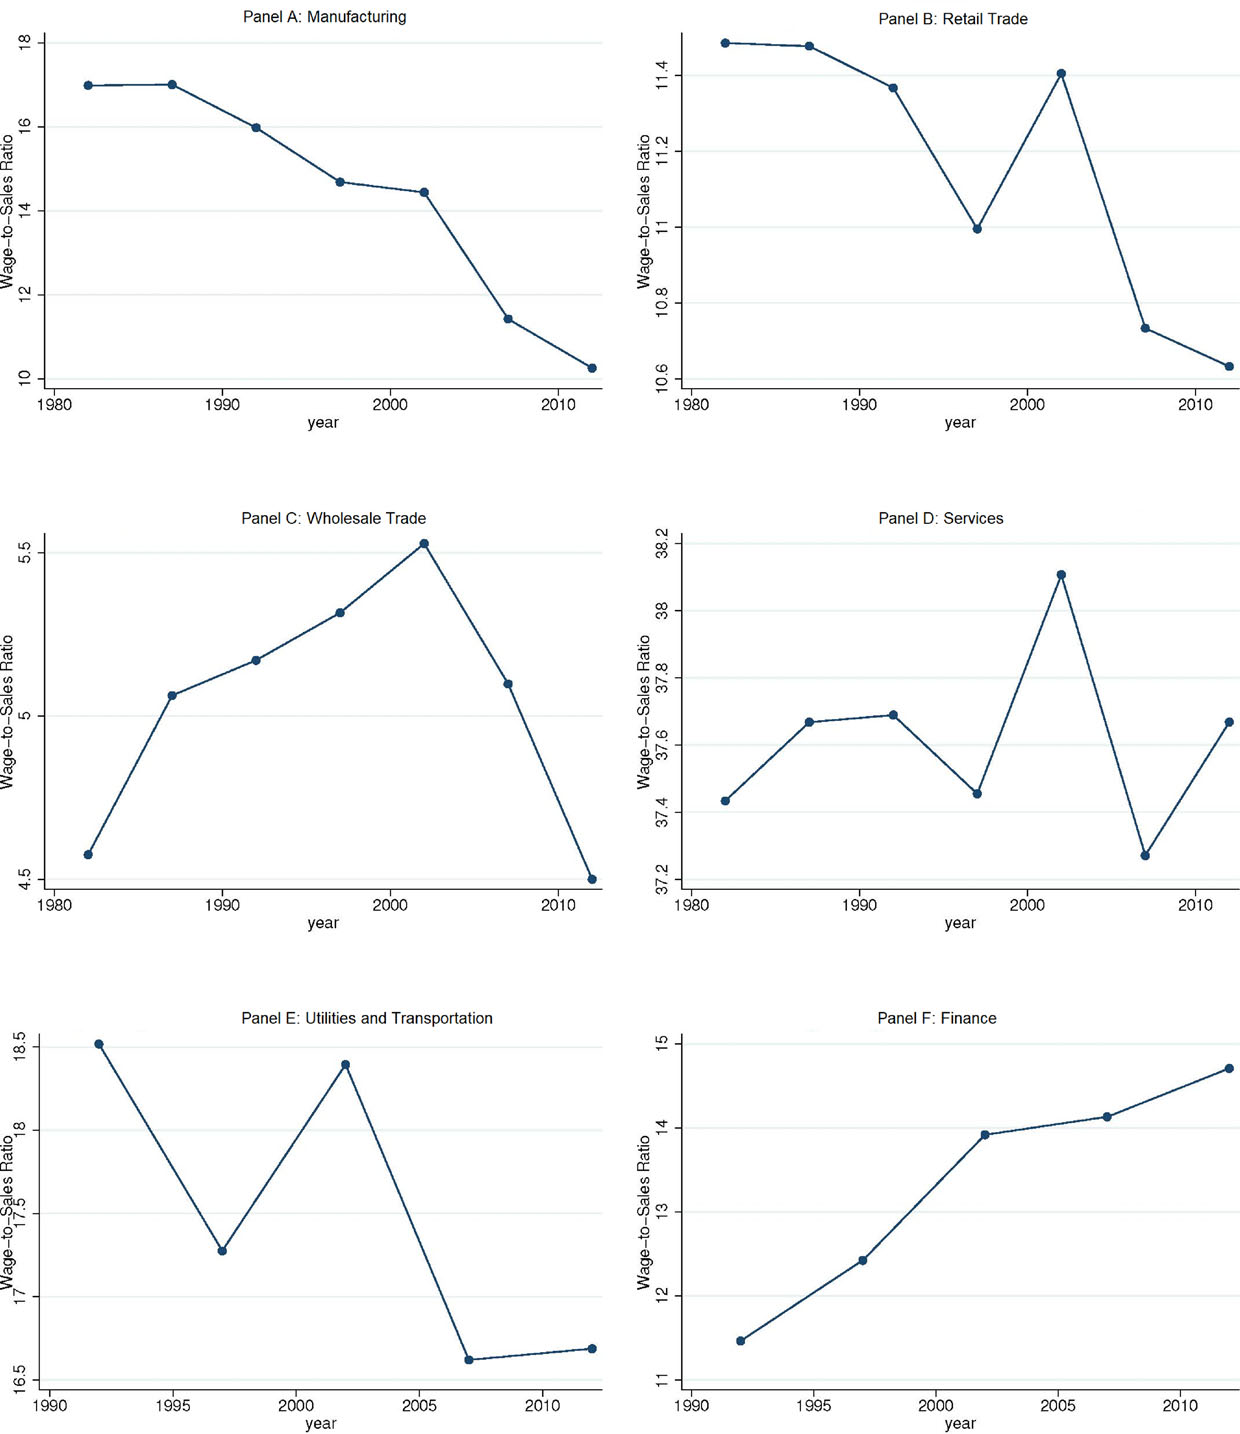
\includegraphics[width=0.6\textwidth,height=\textheight]{./images/Pasted image 20220516203135.png}
\caption{Average Payroll-to-Sales Ratio}
\end{figure}
\end{frame}

\begin{frame}{Finding 1: Concentration}
\protect\hypertarget{finding-1-concentration}{}
\begin{figure}
\centering
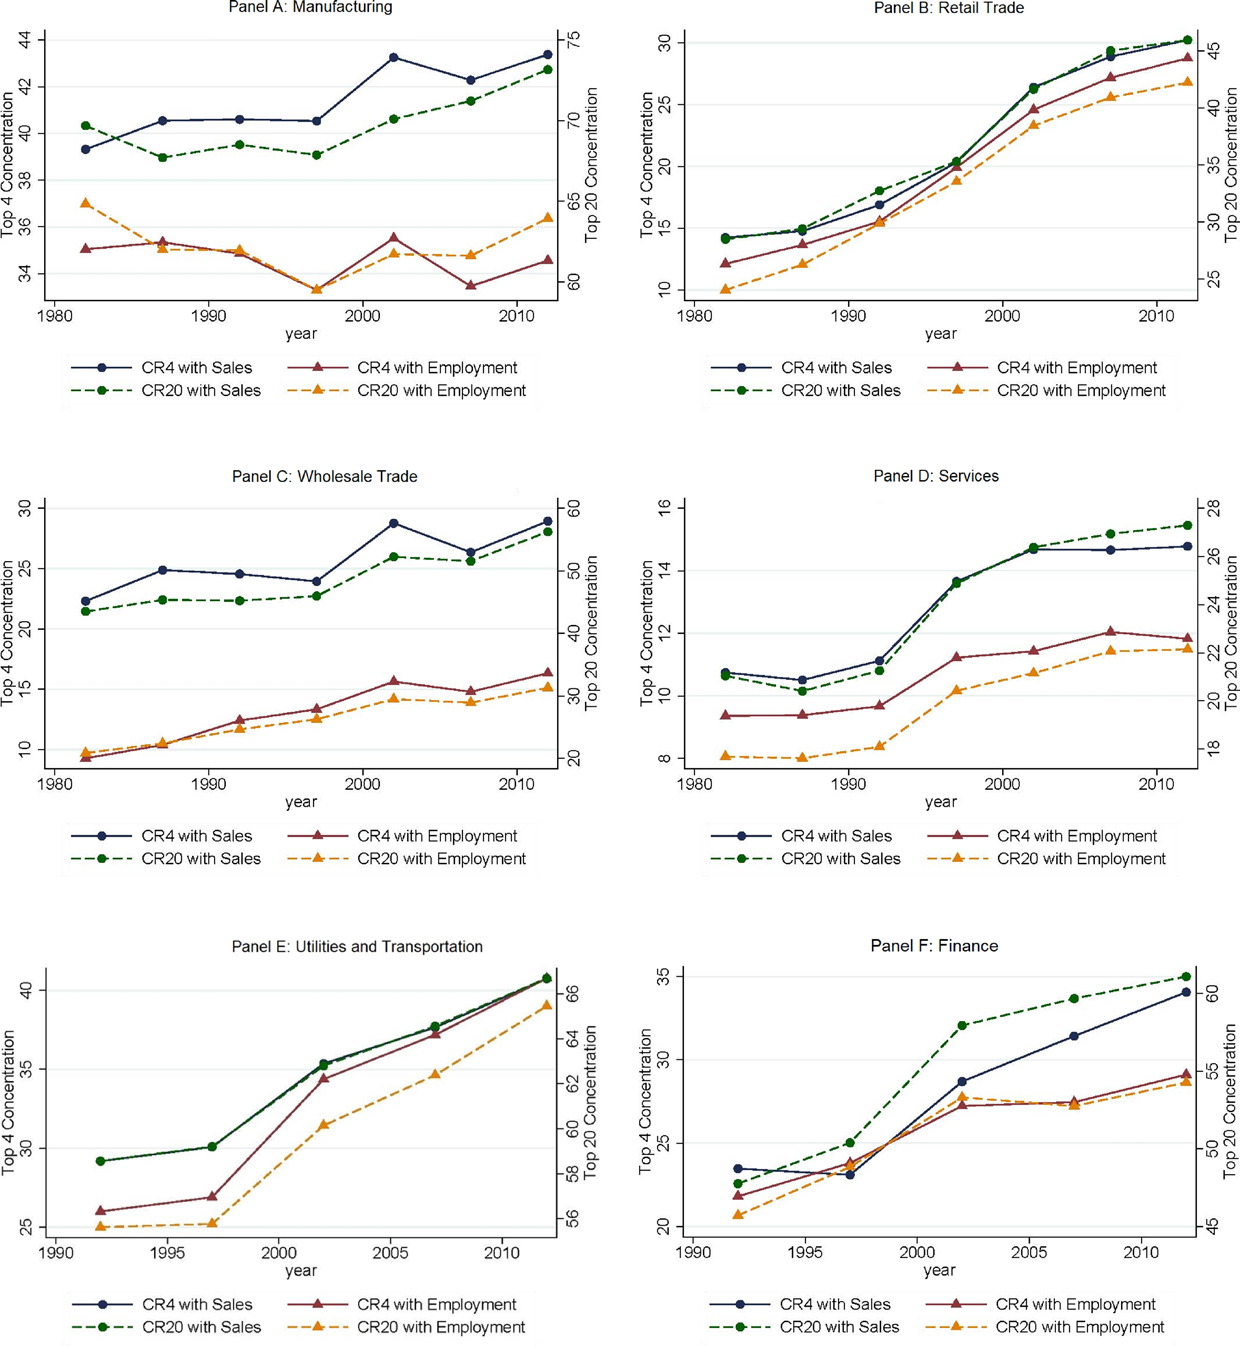
\includegraphics[width=0.65\textwidth,height=\textheight]{./images/Pasted image 20220516204018.png}
\caption{Average Concentration across Four-Digit Industries by Major
Sector}
\end{figure}
\end{frame}

\begin{frame}{Finding 2: Concentration \(\leftrightarrow\) Falling Labor
Shares}
\protect\hypertarget{finding-2-concentration-leftrightarrow-falling-labor-shares}{}
Firm-level regression: labor share on market share

\begin{figure}
\centering
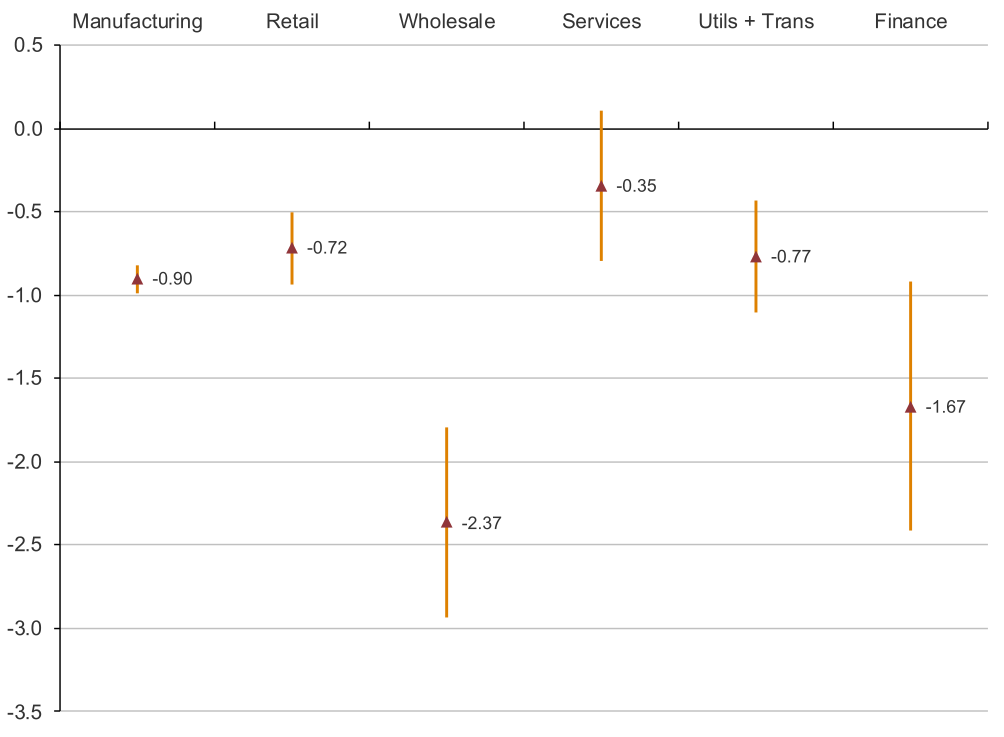
\includegraphics[width=0.8\textwidth,height=\textheight]{./images/Pasted image 20220516204633.png}
\caption{The Relationship between Firm Size and Labor Share}
\end{figure}
\end{frame}

\begin{frame}
Industry-level regression: labor share on concentration index

\begin{figure}
\centering
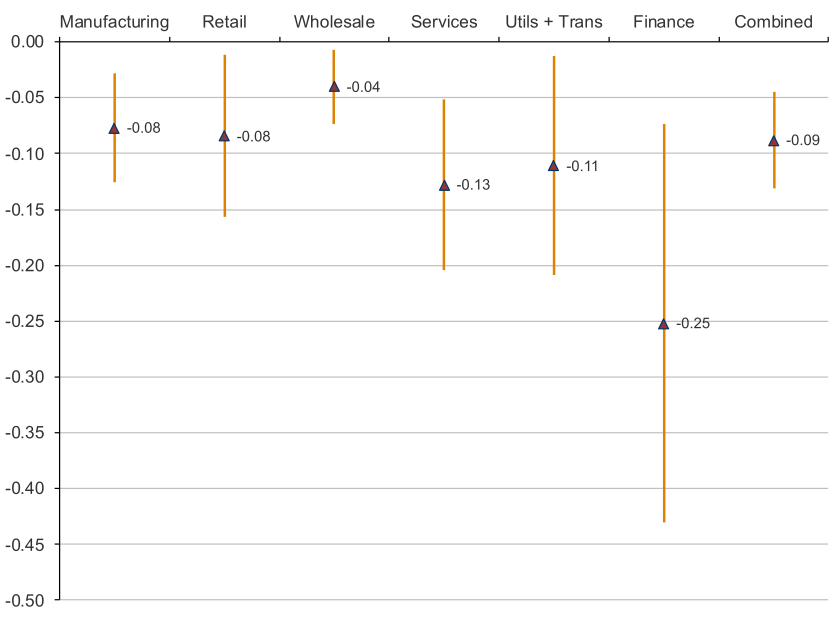
\includegraphics[width=0.8\textwidth,height=\textheight]{./images/Pasted image 20220516205909.png}
\caption{The Relationship between the Change in Labor Share and the
Change in Concentration across Six Sectors}
\end{figure}
\end{frame}

\begin{frame}
Robust for all model settings; Notice impacts of import,
initial-capital.

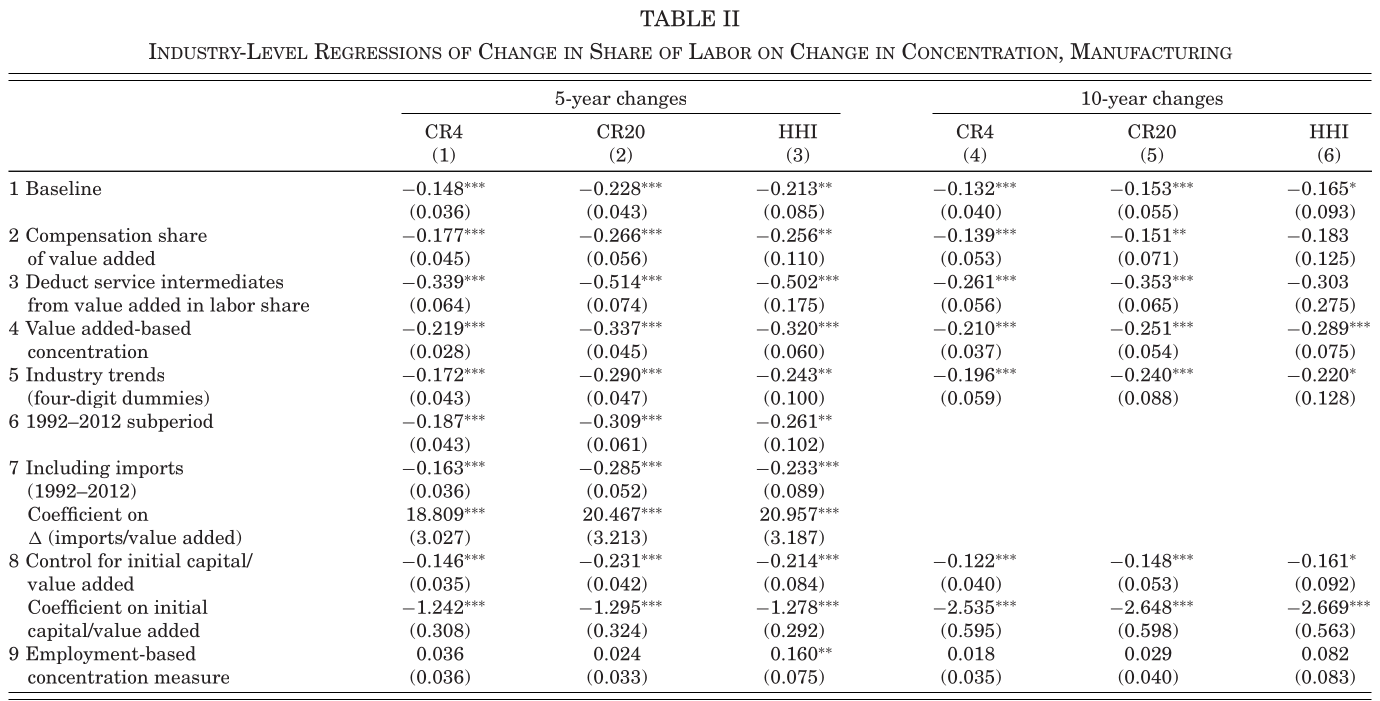
\includegraphics{./images/Pasted image 20220516205229.png}\\
\end{frame}

\begin{frame}
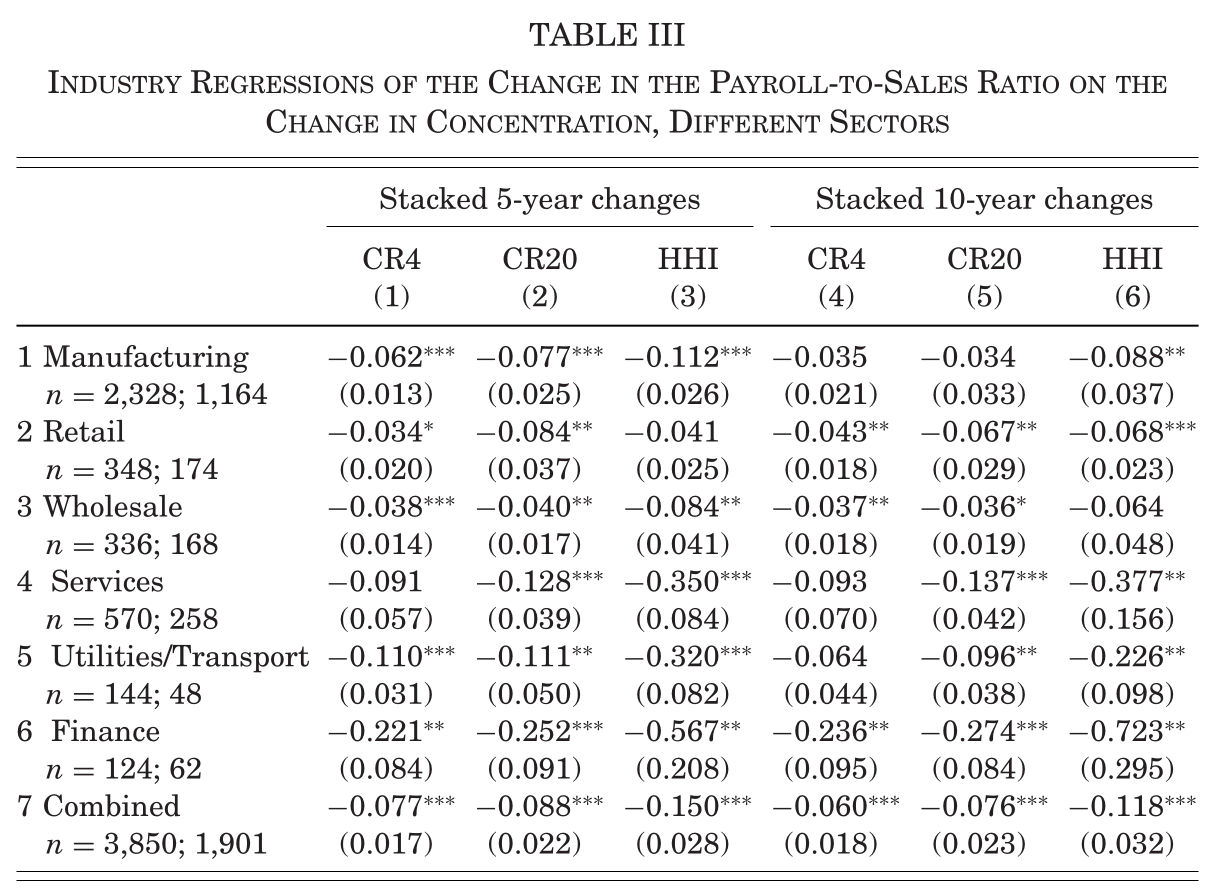
\includegraphics{./images/Pasted image 20220516205438.png}\\
\end{frame}

\begin{frame}{Finding 3: Between-firm Reallocation Dominates}
\protect\hypertarget{finding-3-between-firm-reallocation-dominates}{}
\begin{block}{Decomposition of labor share change}
\protect\hypertarget{decomposition-of-labor-share-change}{}
\[
\begin{aligned}
\Delta S=& \underbrace{\Delta \bar{S}_{S}}_{\text{Within firm }} + \underbrace{\Delta\left[\sum\left(\omega_{i}-\bar{\omega}\right)\left(S_{i}-\bar{S}\right)\right]_{S}}_{\text{Between firm}} + \underbrace{\omega_{X, 0}\left(S_{S, 0}-S_{X, 0}\right)}_{\text{Exiters}} \\
&+ \underbrace{\omega_{E, 1}\left(S_{E, 1}-S_{S, 1}\right)}_{\text{Entrants}}
\end{aligned}
\]
\end{block}
\end{frame}

\begin{frame}
\begin{figure}
\centering
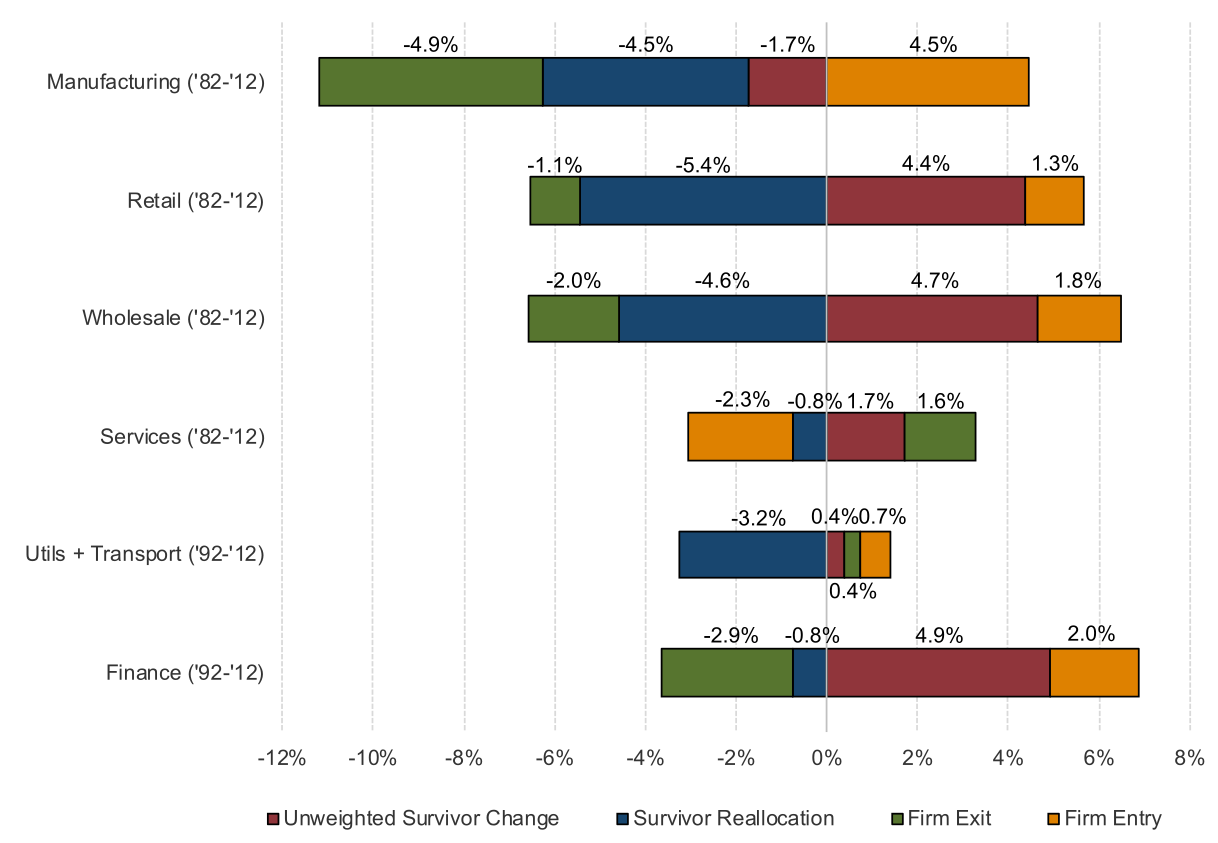
\includegraphics{./images/Pasted image 20220516210943.png}
\caption{Melitz-Polanec Decomposition of the Change in Labor Share in
All Six Sectors}
\end{figure}
\end{frame}

\begin{frame}{Finding 4: Between-Firm Reallocation Is Strongest in
Concentrating Industries}
\protect\hypertarget{finding-4-between-firm-reallocation-is-strongest-in-concentrating-industries}{}
\begin{figure}
\centering
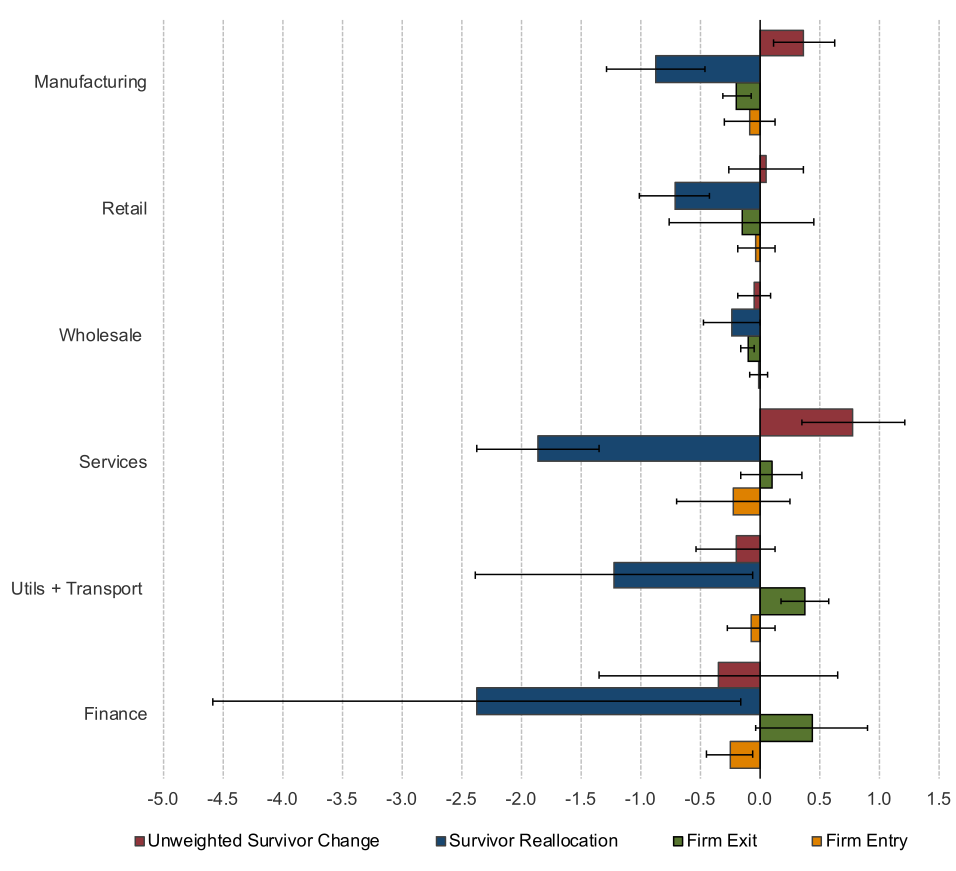
\includegraphics[width=0.7\textwidth,height=\textheight]{./images/Pasted image 20220516211934.png}
\caption{Regressions of the Components of \(\Delta S\) on
\(\Delta\text{Concentration}\)}
\end{figure}
\end{frame}

\begin{frame}{Finding 5: Concentration \(\leftrightarrow\) Innovation \&
Productivity Growth}
\protect\hypertarget{finding-5-concentration-leftrightarrow-innovation-productivity-growth}{}
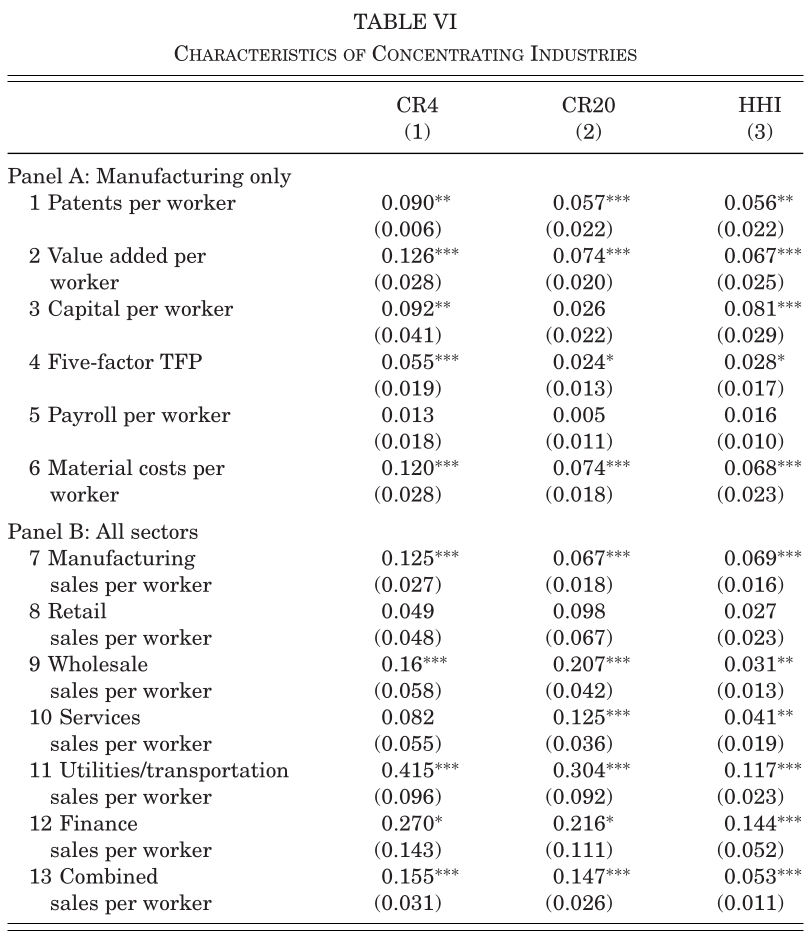
\includegraphics[width=0.9\textwidth,height=\textheight]{./images/Pasted image 20220516212926.png}\\
\end{frame}

\hypertarget{conclusion}{%
\section{Conclusion}\label{conclusion}}

\begin{frame}{Conclusion}
\begin{block}{Conceptual Mechanism}
\protect\hypertarget{conceptual-mechanism}{}
Capital Intensive Competition \(\rightarrow\) Innovative and High
Productivity \(\rightarrow\) Concentration \(\rightarrow\) Superstar
firms \(\rightarrow\) High Markup \(\rightarrow\) Low Labor Share

\begin{itemize}
\tightlist
\item
  Superstar firms might enact barriers to entry to protect their
  positions
\item
  Prevalent labor outsourcing practices
\item
  Future research

  \begin{itemize}
  \tightlist
  \item
    Inequality, outsourcing, part-time job, rank-and-file workers, etc.
  \end{itemize}
\end{itemize}
\end{block}
\end{frame}

\end{document}
